\documentclass[paper=a4, fontsize=11pt]{scrartcl}
\usepackage{amsmath,amsfonts,amsthm}
\usepackage{sectsty}
\usepackage{fourier} % Use the Adobe Utopia font for the document - comment this line to return to the LaTeX default
\usepackage[english]{babel}
\allsectionsfont{ \normalfont\scshape}
\usepackage{fancyhdr}
\usepackage{float}
\usepackage{graphicx}
\usepackage{listings}
\pagestyle{fancyplain}

\fancyhead{} % No page header - if you want one, create it in the same way as the footers below
\fancyfoot[L]{} % Empty left footer
\fancyfoot[C]{} % Empty center footer
\fancyfoot[R]{\thepage} % Page numbering for right footer
\renewcommand{\headrulewidth}{0pt} % Remove header underlines
\renewcommand{\footrulewidth}{0pt} % Remove footer underlines
\renewcommand\floatpagefraction{.9}
\setlength{\headheight}{13.6pt} % Customize the height of the header
\numberwithin{equation}{section} % Number equations within sections (i.e. 1.1, 1.2, 2.1, 2.2 instead of 1, 2, 3, 4)
\numberwithin{figure}{section} % Number figures within sections (i.e. 1.1, 1.2, 2.1, 2.2 instead of 1, 2, 3, 4)
\numberwithin{table}{section} % Number tables within sections (i.e. 1.1, 1.2, 2.1, 2.2 instead of 1, 2, 3, 4)
\setlength\parindent{0pt} % Removes all indentation from paragraphs - comment this line for an assignment with lots of text
\renewcommand{\thesubsection}{\thesection\alph{subsection}}


\setlength\floatsep{1.25\baselineskip plus 2pt minus 2pt}
\setlength\textfloatsep{1.25\baselineskip plus 2pt minus 2pt}



%----------------------------------------------------------------------------------------
%	TITLE SECTION
%----------------------------------------------------------------------------------------

\newcommand{\horrule}[1]{\rule{\linewidth}{#1}} % Create horizontal rule command with 1 argument of height
\title{	
\normalfont \normalsize 
\textsc{Yale-NUS College} \\ [20pt]
\textsc{YID3202C : Data Analysis in Environmental Studies } \\ [25pt] % Your university, school and/or department name(s)
\horrule{0.5pt} \\[0.4cm] % Thin top horizontal rule
\huge Problem Set Four \\ % The assignment title
\horrule{2pt} \\[0.5cm] % Thick bottom horizontal rule
}

\author{Jake Goh Si Yuan} % Your name

\date{\normalsize October 16, 2016} % Today's date or a custom date


\begin{document}

\maketitle % Print the title
\section{Fitting Trends Over the Entire Data Series}
\subsection{}
The average increase of $CO_2$ concentration per year from the linear regression model of $CO_2$ concentration with time(with 1958 as origin) is 1.520, and the average increase per decade is 15.20.

\subsection{}
Taking the time data, with origin 0 set as year 1958 and with year 2016 represented as 58, we will arrive at a nominal start-point of 307ppm and endpoint of 395.16ppm\\

The start-point of the data is 315.71ppm or 8.71ppm higher than trend-predicted, and the end-point is 402.25ppm or 7.19ppm higher.
\subsection{}

The standard deviation of the data-misfit residual, or the residual standard error, is 3.871 on 700 degrees of freedom. The F variance ratio, or statistic, is 30880.
\pagebreak
\subsection{}
\begin{figure}[htp]
	\centering
	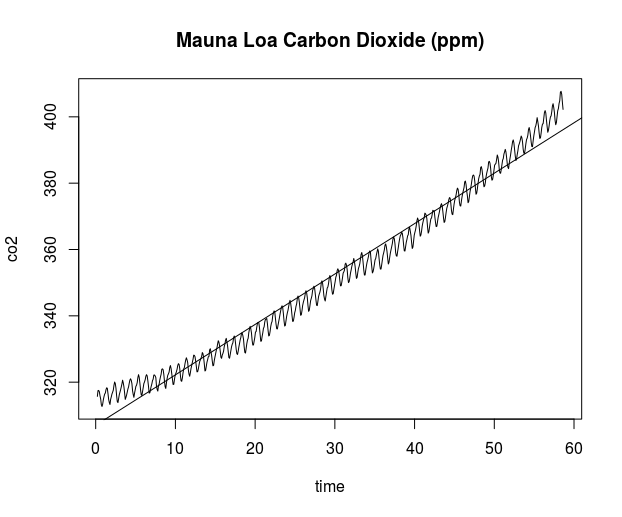
\includegraphics[width=0.7\textwidth, clip]{q1aTime.png} 
	\caption{Linear regression of time(with 1958 as origin) and Mauna Loa Carbon Dioxide}
\end{figure}

The data does not seem to follow strictly to a straight line, in fact, it appears to be have an exponential trend with a small enough exponent that it takes on pseudo-linear characteristics.\\

Also, the linear prediction fails to take into account the saw-tooth motion that the data is taking, or the trend within the trend.

\subsection{}

The predicted start-point for the quadratic model is 314.2ppm, as compared to the actual start-point of 315.71ppm, with a difference of -1.51ppm.

The predicted end-point is 401.89ppm, as compared to the actual end-point of 402.25ppm, with a difference of -0.36ppm.

\subsection{}
The predicted yearly increase at the start-point of the quadratic model is 0.8055ppm, and at the end-point it is 
2.235ppm.

\subsection{}
The standard deviation of the data-misfit residual, or the residual standard error, is 2.209 on 699 degrees of freedom. The F variance ratio, or statistic, is 48160.

\subsection{}

\begin{figure}[htp]
	\centering
	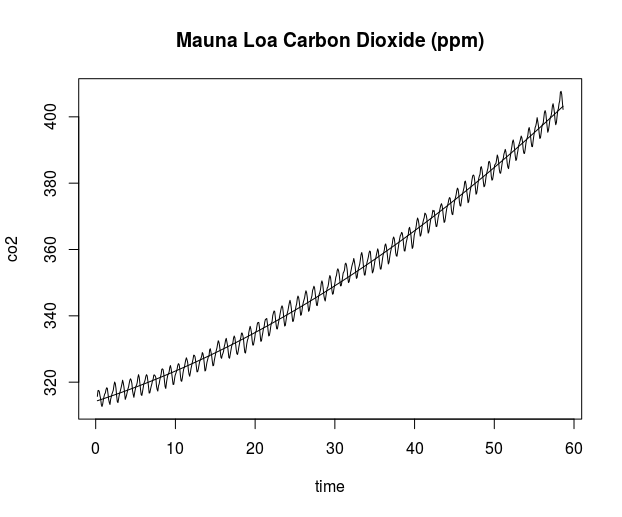
\includegraphics[width=0.7\textwidth, clip]{q1hTime.png} 
	\caption{Quadratic regression of time(with 1958 as origin) and Mauna Loa Carbon Dioxide}
\end{figure}

The quadratic model offers a better fit as compared to the linear model. We can look at the comparisons between predicted start-point/endpoint and actual start-point/endpoint to see that the error has become much smaller. \\

However, the big inherent problem of not being able to take into account of the saw-tooth motion is still present. \\

Although the quadratic model is able to help us reject a linear model, we do not know if the global trend is indeed quadratic-like, or if it is only localized to the 58 years frame.

\subsection{}
 
The standard deviation of the data-misfit residual, or the residual standard error, is 2.21 on 699 degrees of freedom.\\

The significance of the cubic parameter is 0.642, which means that it is not very significant, and the null hypothesis of not having a cubic parameter cannot be rejected.

\section{Fitting Trends and Cycles Over the Entire Data Series}

\subsection{}

The amplitude of the annual cycle in $CO_2$ is $2.833\pm0.06967$ ppm.

\subsection{}

The annual maximum occurs at 0.3095 of the cycle, or approxmiately towards the end of April. A quick sanity check at a zoomed in slice roughly confirms the assertion.

\begin{figure}[htp]
	\centering
	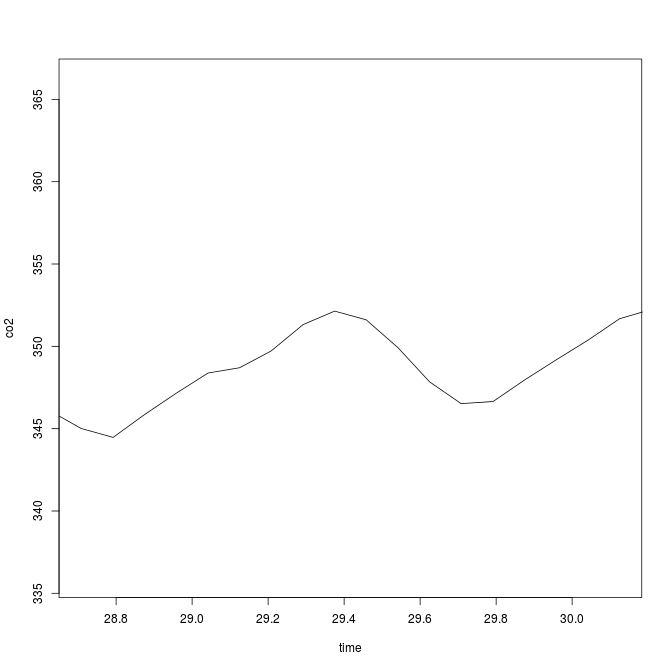
\includegraphics[width=0.7\textwidth, clip]{q2bZoom.png} 
	\caption{Zoomed in slice of time(with 1958 as origin) and Mauna Loa Carbon Dioxide}
\end{figure}
\pagebreak
\subsection{}

\begin{figure}[htp]
	\centering
	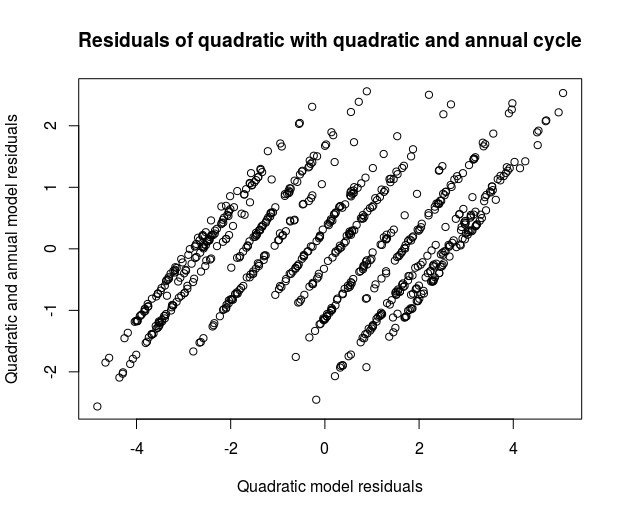
\includegraphics[width=0.7\textwidth, clip]{q2c.png} 
	\caption{Comparing quadratic model residuals with quadratic and annual cycle residuals}
\end{figure}

The standard deviation of the quadratic model only is 2.206 whilst the standard deviation of the quadratic model and annual cycle residuals is 2.064.


\subsection{}

The amplitude of the semi-annual cycle of $CO_2$ is $0.7814\pm0.055805$ ppm.

The inclusion of the semi-annual cycle gives the model a sharper characteristic in terms of the reverse in trend in the annual cycle. In other words, when maxima or minima is arrived at during the annual cycle, the first derivative changes direction much faster.

The amplitudes of maximum and minimum also increase by approximately $10\%$.

\pagebreak

\subsection{}
\begin{figure}[htp]
	\centering
	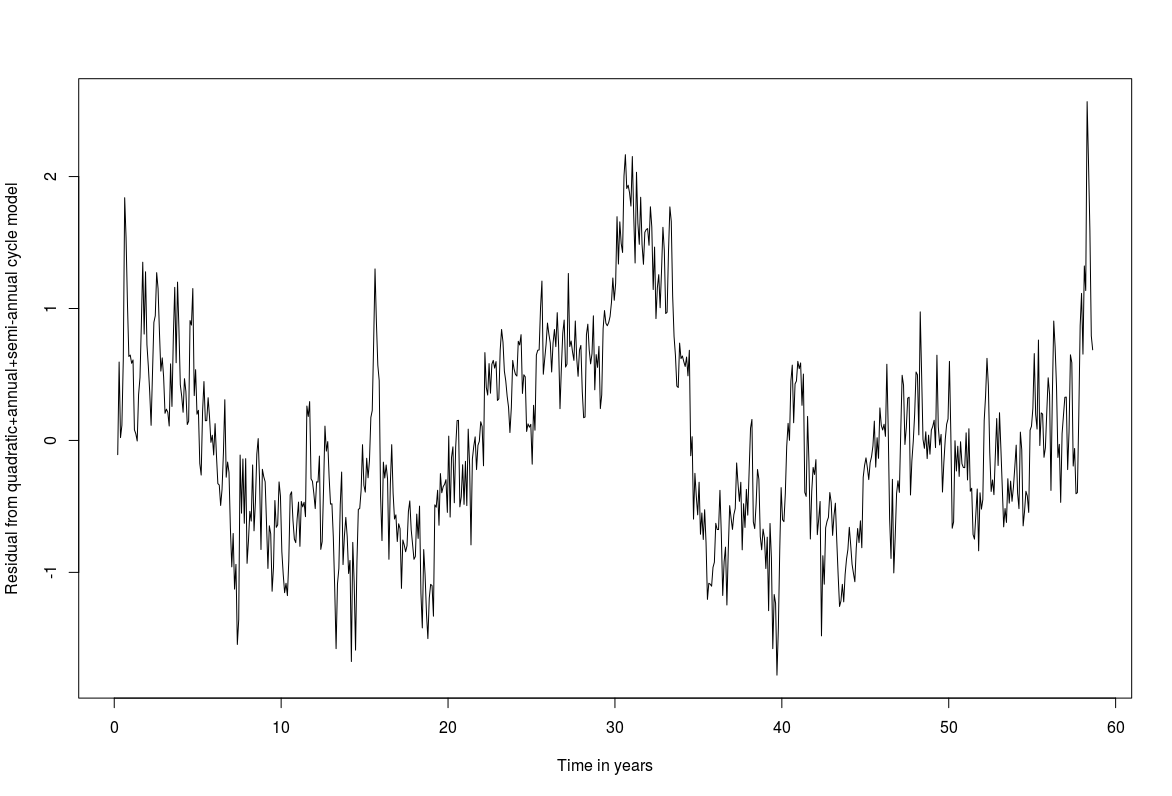
\includegraphics[width=0.7\textwidth, clip]{q2e.png} 
	\caption{Residuals from quadratic, semi-annual and annual model with time}
\end{figure}
The standard deviation is 0.7361.

\pagebreak
\section{Fitting Trends and Cycles Over 10-year Data Segments}

\subsection{}

\begin{figure}[htp]
	\centering
	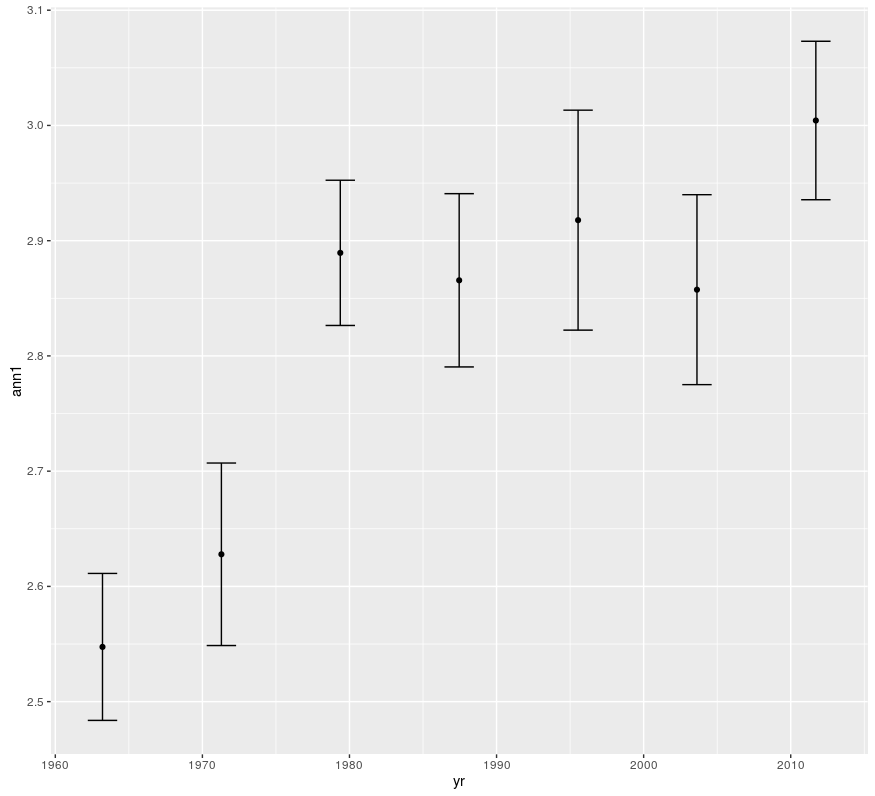
\includegraphics[width=0.7\textwidth, clip]{q3a.png} 
	\caption{Annual-cycle amplitudes for decade-long segments of Mauna Loa $CO_2$ time series}
\end{figure}
There is definitely an upward trend in the annual-cycle amplitudes. However, this trend at first glance does not appear to follow a simple model(linear, quadratic or otherwise).
\\

The trend can be best described with two characteristics:\\
1. A sharp transitional increase from 1970 - 1980.


2. Slow but steady increase between 1980-2010.

\pagebreak
\subsection{}

\begin{figure}[htp]
	\centering
	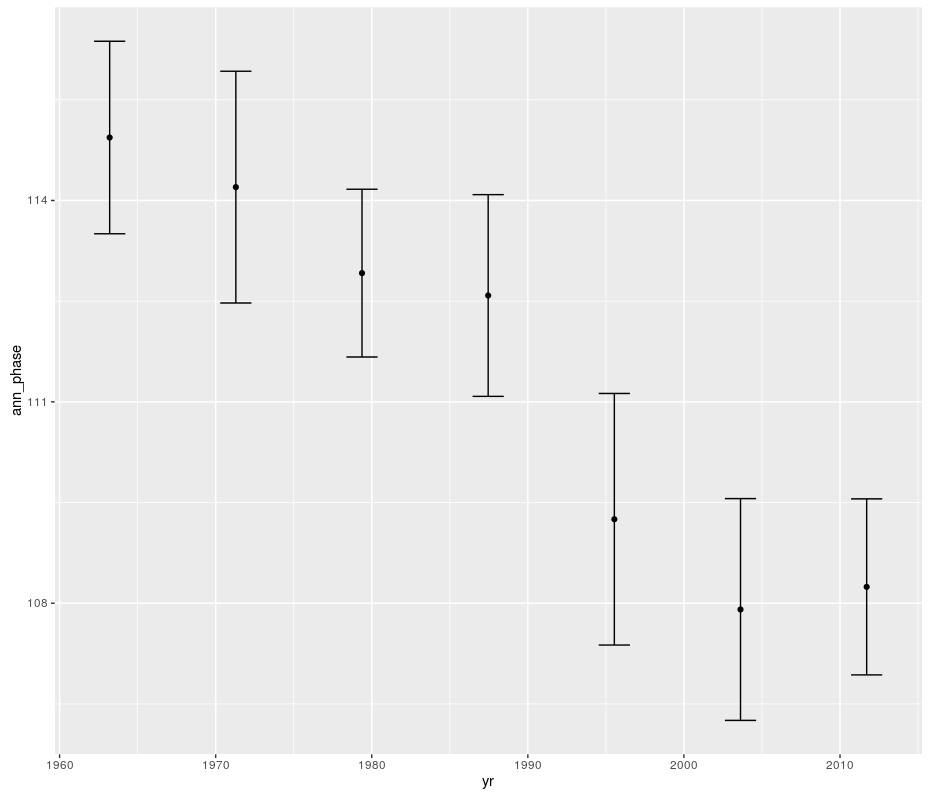
\includegraphics[width=0.7\textwidth, clip]{q3b.png} 
	\caption{Annual-cycle phases for decade-long segments of Mauna Loa $CO_2$ time series}
\end{figure}
The days have shifted by approximately $6.695\pm 2.745$ days.

\pagebreak
\subsection{}
\begin{figure}[htp]
	\centering
	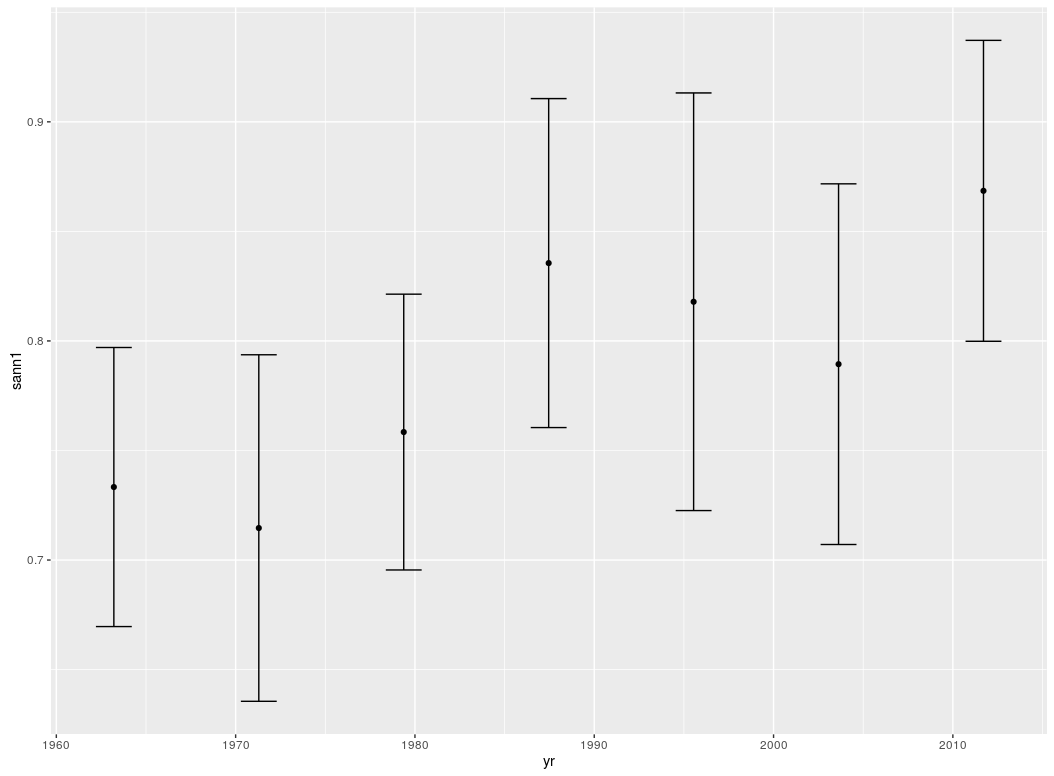
\includegraphics[width=0.7\textwidth, clip]{q3c.png} 
	\caption{Semi-annual-cycle amplitudes for decade-long segments of Mauna Loa $CO_2$ time series}
\end{figure}
The semi-annual amplitudes follow a slow increasing trend from 1958 to 2010, from a starting point of 0.733 to a final maximum endpoint of 0.8685. 

Interestingly, the starting point is not the minima of the graph, although that can be easily explained by the high error bars, and the negligible distance(in y and x axis) between the minimum and the starting point.

Just like in the annual trend, there is a sharper increase between 1970-1980, although in this case it goes on further towards 1990, before taking a small decline until the mid of 2000 and 2010, before reversing in trend and making a sharp increase to 2010 and onwards.

\pagebreak
\section{Fitting an Exponential Trend Over the Full Data Series}
\subsection{}
\begin{figure}[htp]
	\centering
	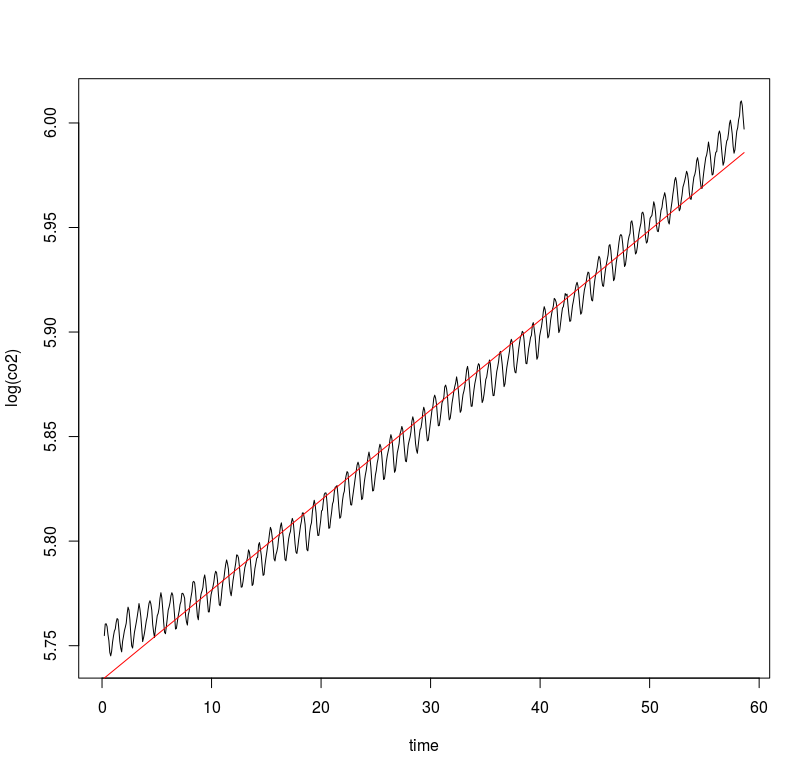
\includegraphics[width=0.7\textwidth, clip]{q4a.png} 
	\caption{Logarithmic version of exponential model of Mauna Loa}
\end{figure}
\pagebreak
\subsection{}
\begin{figure}[htp]
	\centering
	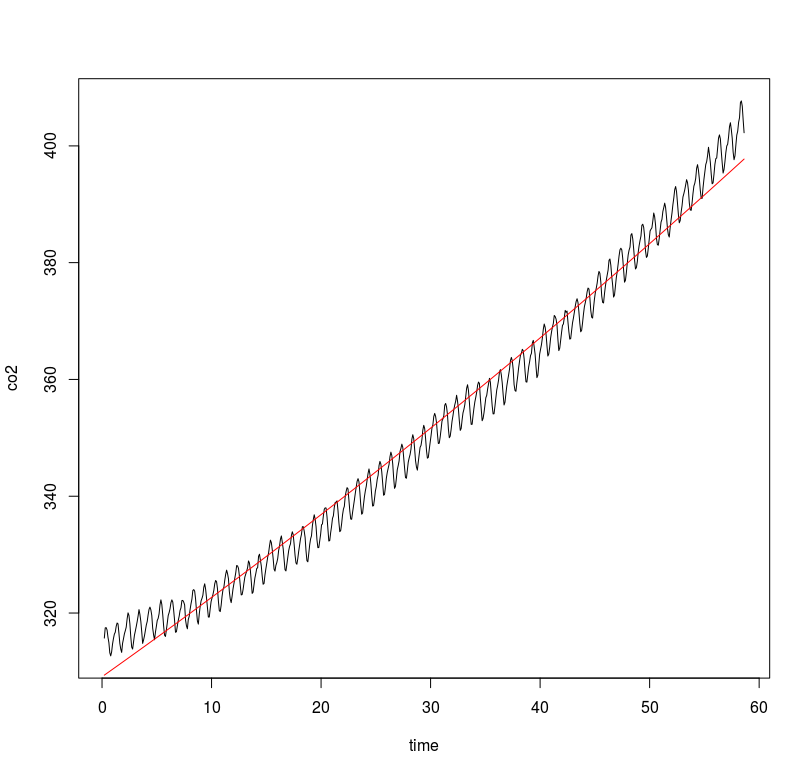
\includegraphics[width=0.7\textwidth, clip]{q4b.png} 
	\caption{Exponential model of Mauna Loa}
\end{figure}

The value at 1958 is 309.36 and the value at 2016 is 397.74.

The data fit fails to take into account the semi-annual and annual cycle, and provides a seemingly poor prediction for the start and end-points.

For an exponential model, this appears very linear, and it is no surprise given that the method employed begins with a linear modelling through the logarithmic before converting back by exponentiating.
\pagebreak
\subsection{}
\begin{figure}[htp]
	\centering
	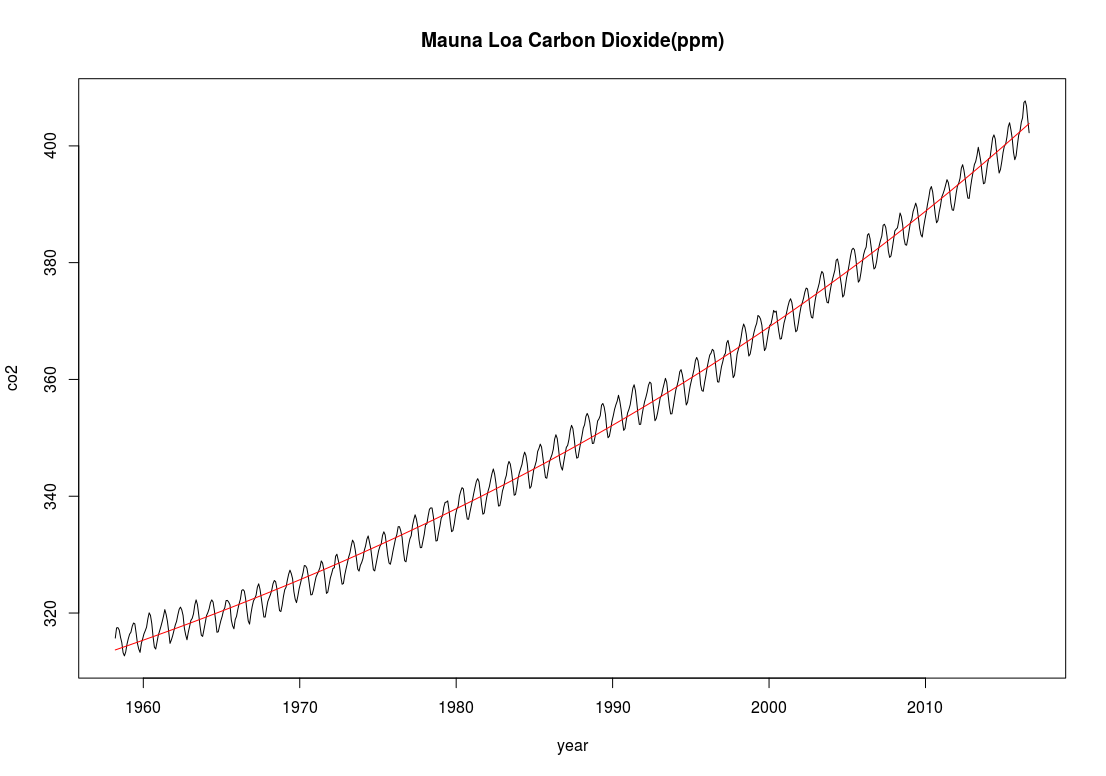
\includegraphics[width=0.7\textwidth, clip]{q4c.png} 
	\caption{Exponential model of Mauna Loa with nls}
\end{figure}

The value for A is $256.9\pm2.542$, the value for B is $56.61\pm2.357$ and the value for C is $0.01627\pm0.0004390$.

The standard error of residual is 2.225 on 699 degrees of freedom.

This model bears a remarkabe similarity to the quadratic-polynomial solution.

\subsection{}
The standard deviation of 280 from A is 9.087.

We get an extrapolation of 260.46ppm.






















\end{document}